%% Developing a solution for multimedia home networking chapter
%% author Liu Peng

To fulfill the need of interoperability among devices in home networking,
Tuxera Inc. started a project named Streambels(later renamed as AllConnect). The
project aims to solve the interoperability issue in multimedia home networking
by making a universal solution that can connect all available devices at home
and make them work together regardless of what protocol they use.\\
\\
Most devices at home are embedded solutions and have their own firmwares, it is
hard to update or even impossible to upgrade the software running on these
devices. On the other hand, most home network users
 are not knowledgeable enough to 
to manually set up the more advanced
 network features to achieve certain degree of device interoperability. Plus
 most of these network infrastructures are not designed to be easily
 configured. Due to these reasons, building interoperability among different
 devices through a mobile device seems to be the most straightforward solution,
 for mobile devices can serve as a very flexible and programmable portal for
 home-networking.  Other advantages of mobile devices include their great
 processing power, networking capabilities and their wide adoption and
 availability. Through the available platforms and tools, a mobile application
 could possibly be developed to control all multimedia streaming data flows and
 act as a personal access portal for home networking.\\
\\
After a year of development, our team have built up an Android application that
can be used to control and connect every known type of multimedia device at home.
Encouragingly, the number of our application users have grown to nearly one
million so far, providing a strong proof of the effectiveness of our solution.

\subsection{Architecture overview}
In order to solve the multimedia home networking interoperability problem, the system should be designed to control media playback sessions. Consequently, content navigation, manage receiver device, and media playback should be the most important three components. In our solution, the system architecture consists of three major parts: device discovery, content management and streaming.\\
\\
Discovery component is responsible for device discovery. As discussed
in\ref{upnp}, UPnP devices and DIAL devices use Simple Service Discovery Protocol for device discovery. An application firstly send a M-Search request over UDP to the IPv4 multicast address 239.255.255.250 and UDP port 1900. Then the application listens to other devices' response. A DIAL device will return a response with Application URL header, while the UPnP/DLNA devices will return a message with a XML body, which gives detailed service URL and description URL. On the other hand, Apple's products use Multicast DNS is for discovery. \\
\\
For the three protocols we are planning to support, we need to implement two kinds of discovery mechanism: Simple Service Discovery Protocol(SSDP) and Multicast DNS protocol.\\
\\
Content management component is responsible for organizing and
navigating multimedia contents which can be found in the home network. In our solution, these content sources include both phone's local storage and DLNA digital media servers that are connected to home network. Content from these sources could be streamed using all of the
three protocols that we support.\\
\\
Streaming component is responsible for streaming multimedia content to the selected multimedia receivers, such as TVs, wireless speakers, set top boxes. Since DLNA, AirPlay video/ photo and Chromecast all use HTTP streaming, while AirPlay music uses Remote Audio Output Protocol (RAOP). In our solution, two types of media server are built inside our application. A RAOP server will handle the AirPlay music streaming and a HTTP media server will handle the streaming of all the other solutions.

\subsection{Implementation}
Since the application is built upon Android platform, we studied Android system architecture and Android Software Development Kit (SDK). Fortunately, Android SDK provides many useful Application Programming Interfaces (APIs) and gives crucial permissions to access hardware features, such as accessing Internet, accessing WiFi state change, allowing WiFi multicast, reading phone storage. The programming language used in developing Android Application is Java, however some CPU-intensive work such as transcoding have to be implemented in C and embed to the application using Android Native development kit (NDK).\\
\\
While Apple has not provided its official specification of AirPlay, the implementation of AirPlay is mostly written following the unofficial guidelines. However, Apple provide its official Multicast DNS (mDNS) implementation. This piece of code is reused and compiled as a shared native library. Remote Audio Output Protocol (RAOP) is
implemented according to the unofficial guidelines. The implementation includes a UDP server and TCP control channel.\\
\\
DLNA has open specification only for its members. Tuxera is a member of DLNA so we got detailed specification and test tools. Since DLNA is a popular standard, there are a lot of open source UPnP/DLNA
libraries. In our implementation, we used a library called "cling"\cite{cling}, it has minimal implementation of UPnP
device discovery, description information parsing, and basic message handling. More code is written by us to ensure the media format compatibility across different devices.\\
\\
Google has officially provided Chromecast SDK for different mobile platforms, so integration with Chromecast becomes trivial. In Streambels project, the Chromecast integration is built upon Chromecast API.\\
\\
When it comes to media server implementation, according to the DLNA guideline,
certain additional headers need to be implemented in the stream. This
requirement demand the HTTP server to be flexible to add DLNA specific
headers. Another requirement is that "Seek" action needs to be supported on the server side, in the implementation we need to enable byte based seeking operation.\\
\\
For receivers other than DLNA standard, a basic file server with byte range support will be sufficient to do the work.\\
\\
In order to serve media for all the receivers from both online and local storage, a separate media proxy also needs to be implemented.\\
\\
After investigating and comparing multiple server implementations on Android, we
concluded that NanoHTTPD is the ideal solution for our need. It is easy to use,
Apache licensed, very tiny and efficient implementation. Because it is minimal implemented, it is also easy to be modified. Additional headers can be easily added to be compatible with DLNA receivers. Besides, a proxy is also easy to integrate with the NanoHTTPD.\\
\\
Taking all these technical details into consideration, we concluded a simplified
architecture of our implementation, which is shown in the Figure \ref{chart3}.
\begin{figure}[htb]
\centering 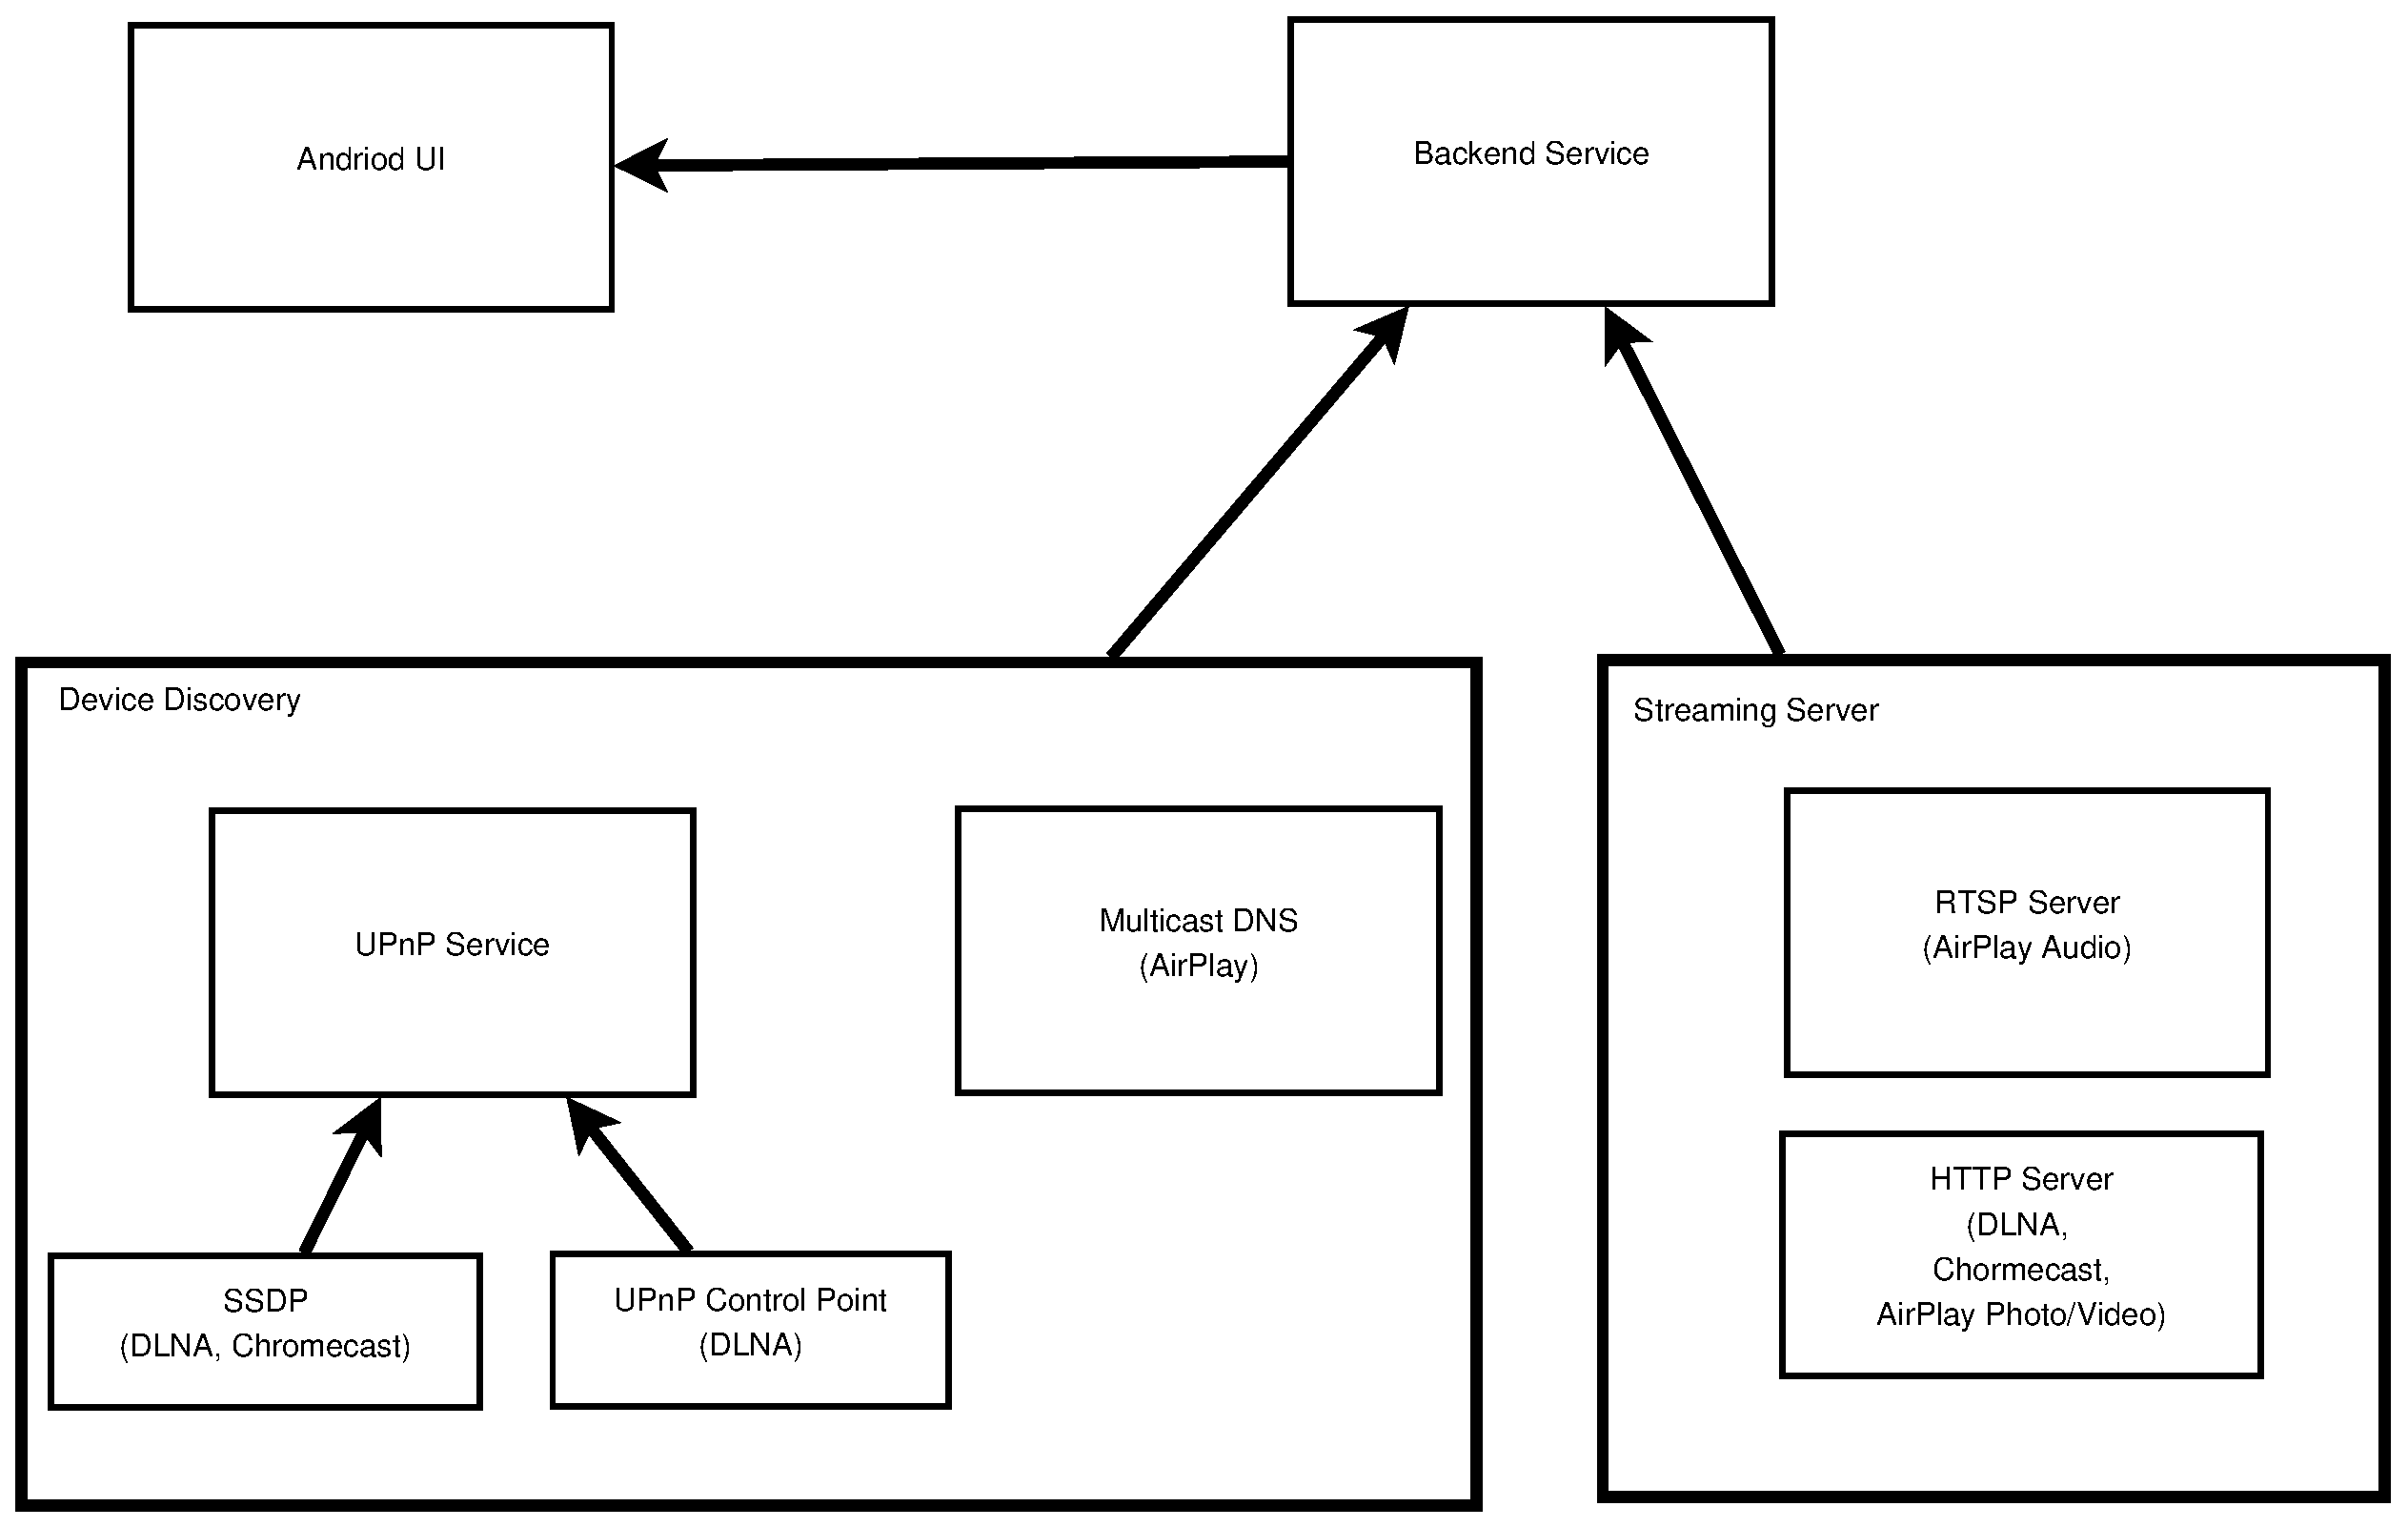
\includegraphics[height=9cm]{charts/chart3}
\caption{Simplified application architecture\label{chart3}}
\end{figure}

When streaming content, the data flow can be described in three different models. Figure \ref{chart4} shows the following three use scenarios:\\
\\ 
If the content is stored in mobile phone, a streaming server in the application will be used to stream the content from phone to selected receiver.\\
\\
Otherwise, if the content is located on Internet and the receiver is a DLNA Media Renderer, a proxy will be needed. The proxy will firstly download the resource stream, then add the required headers by DLNA specification and finally stream the modified content to the selected DLNA Media Renderer.\\
\\
Finally, if the streamed content locates in a DLNA Digital Media Server, then the source can be used directly by all receivers. In this case, the streaming proceeds directly from media server to receivers. Application will only be used as a control point and do not participate in the media transmission in this scenario.\\
\\
\begin{figure}[htb]
\centering 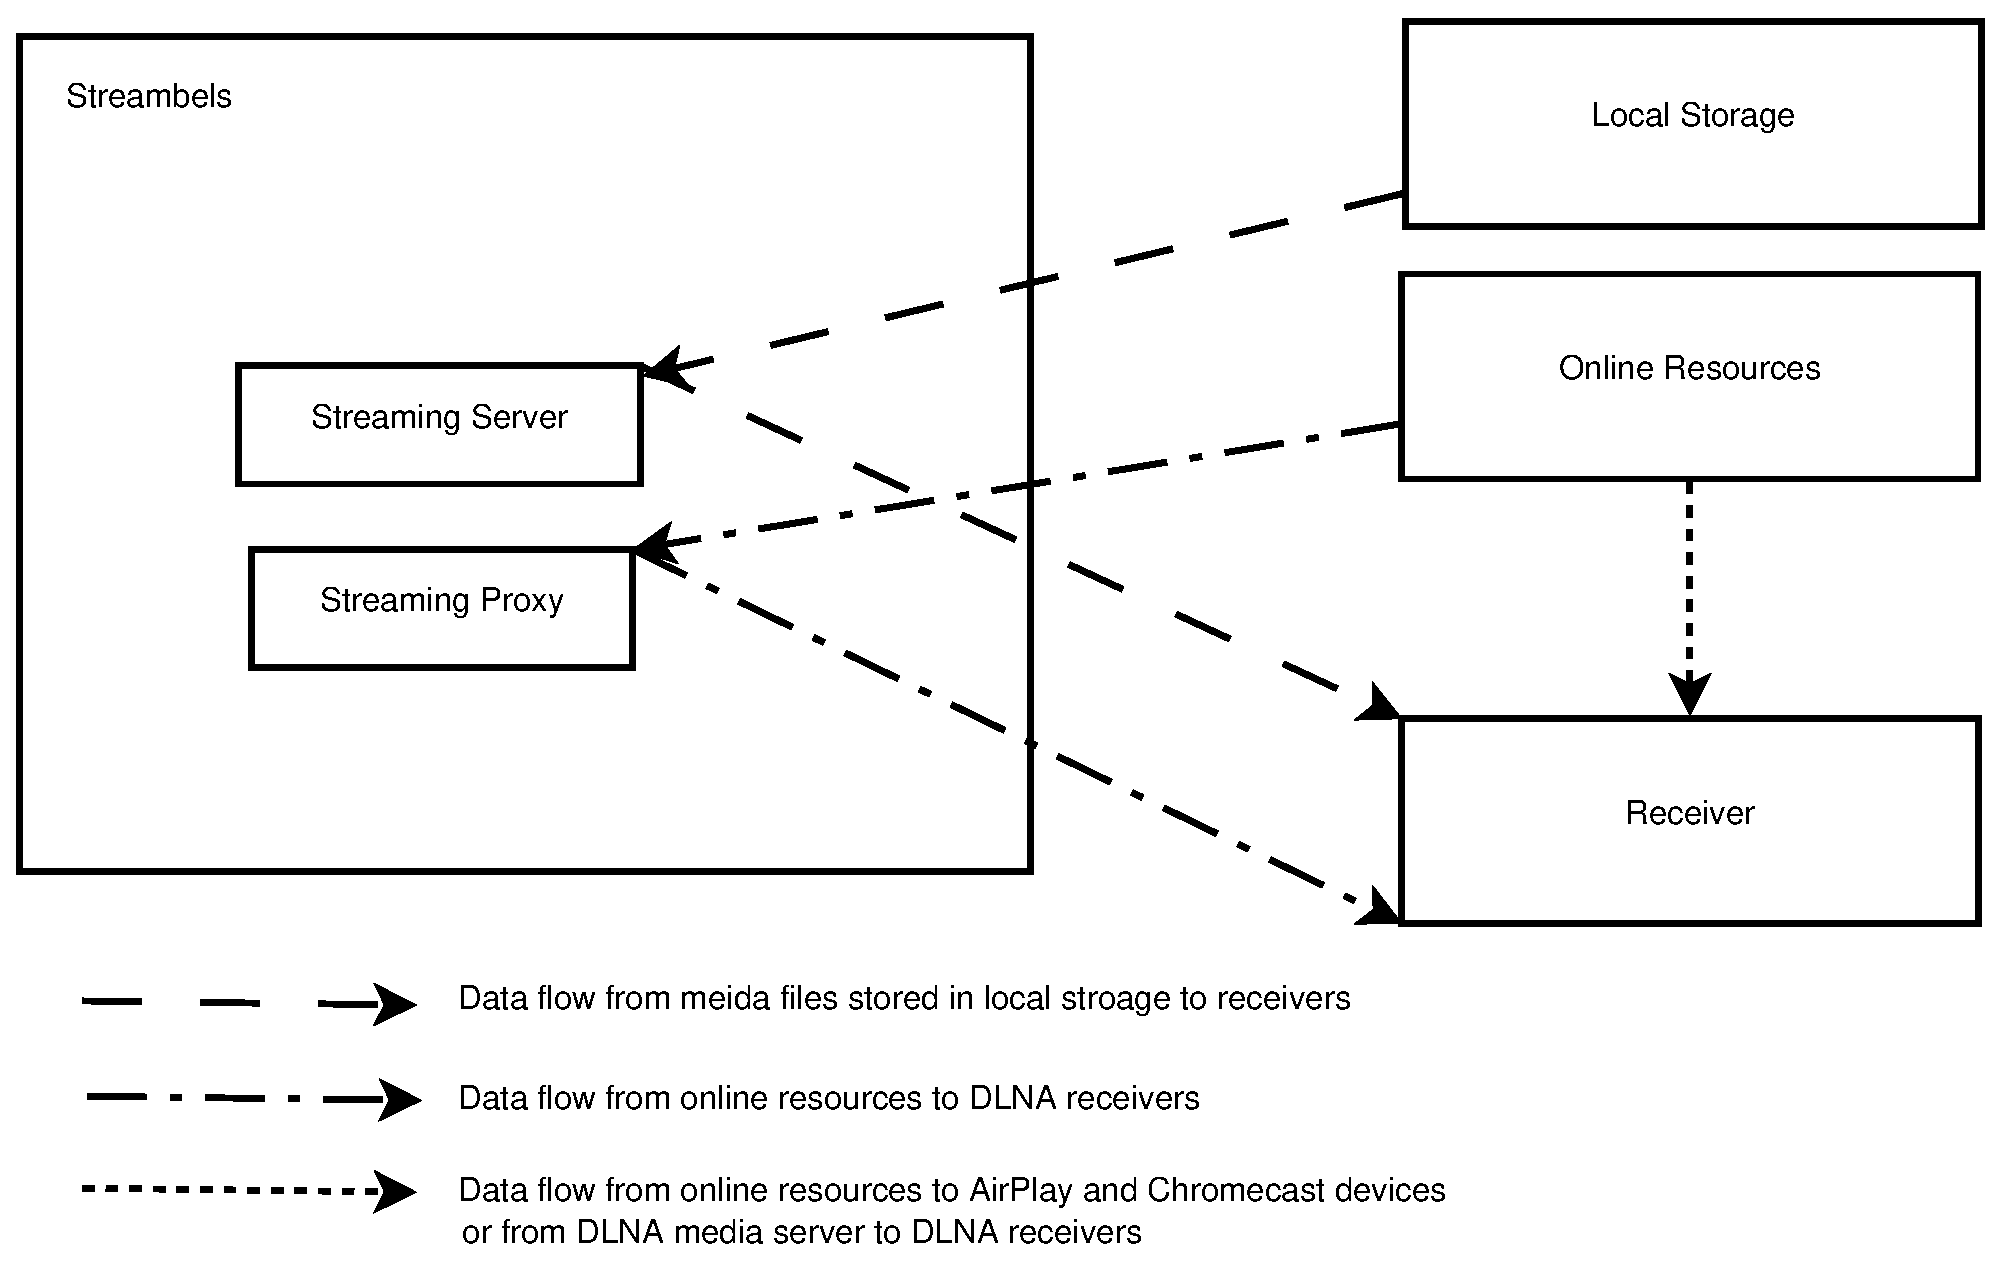
\includegraphics[height=9cm]{charts/data_flow}
\caption{Simplified data flow \label{chart4}}
\end{figure}

\subsection{UX design}
In terms of UI and UX, the application should be simple enough to be used by everyone. Users should be able to locate the media, browse
content on different sources, and follow the data flow between devices without any difficulty. The control of different devices should also be intuitive so that the interoperation between different devices goes seamlessly.\\
\\
A multimedia home networking solution should be content centric so that user can easily navigate through different sources. The application is designed similar to a multimedia player. A cast button is added at the top of the application to make it easier to select cast devices. The content is categorized into 4 sections: music, video, photo and online sources. In Android, since the system provides share intent method for inter-activity communication, an interface is also made to manage share intents from other activities. The selected receiver is designed to be visible to user from everywhere inside the application. \\
\\
Having all these considerations in mind, the final appearance of the application becomes simple but effective. Figure \ref{chart5} shows the final design of our application.
\begin{figure}[htb]
\centering 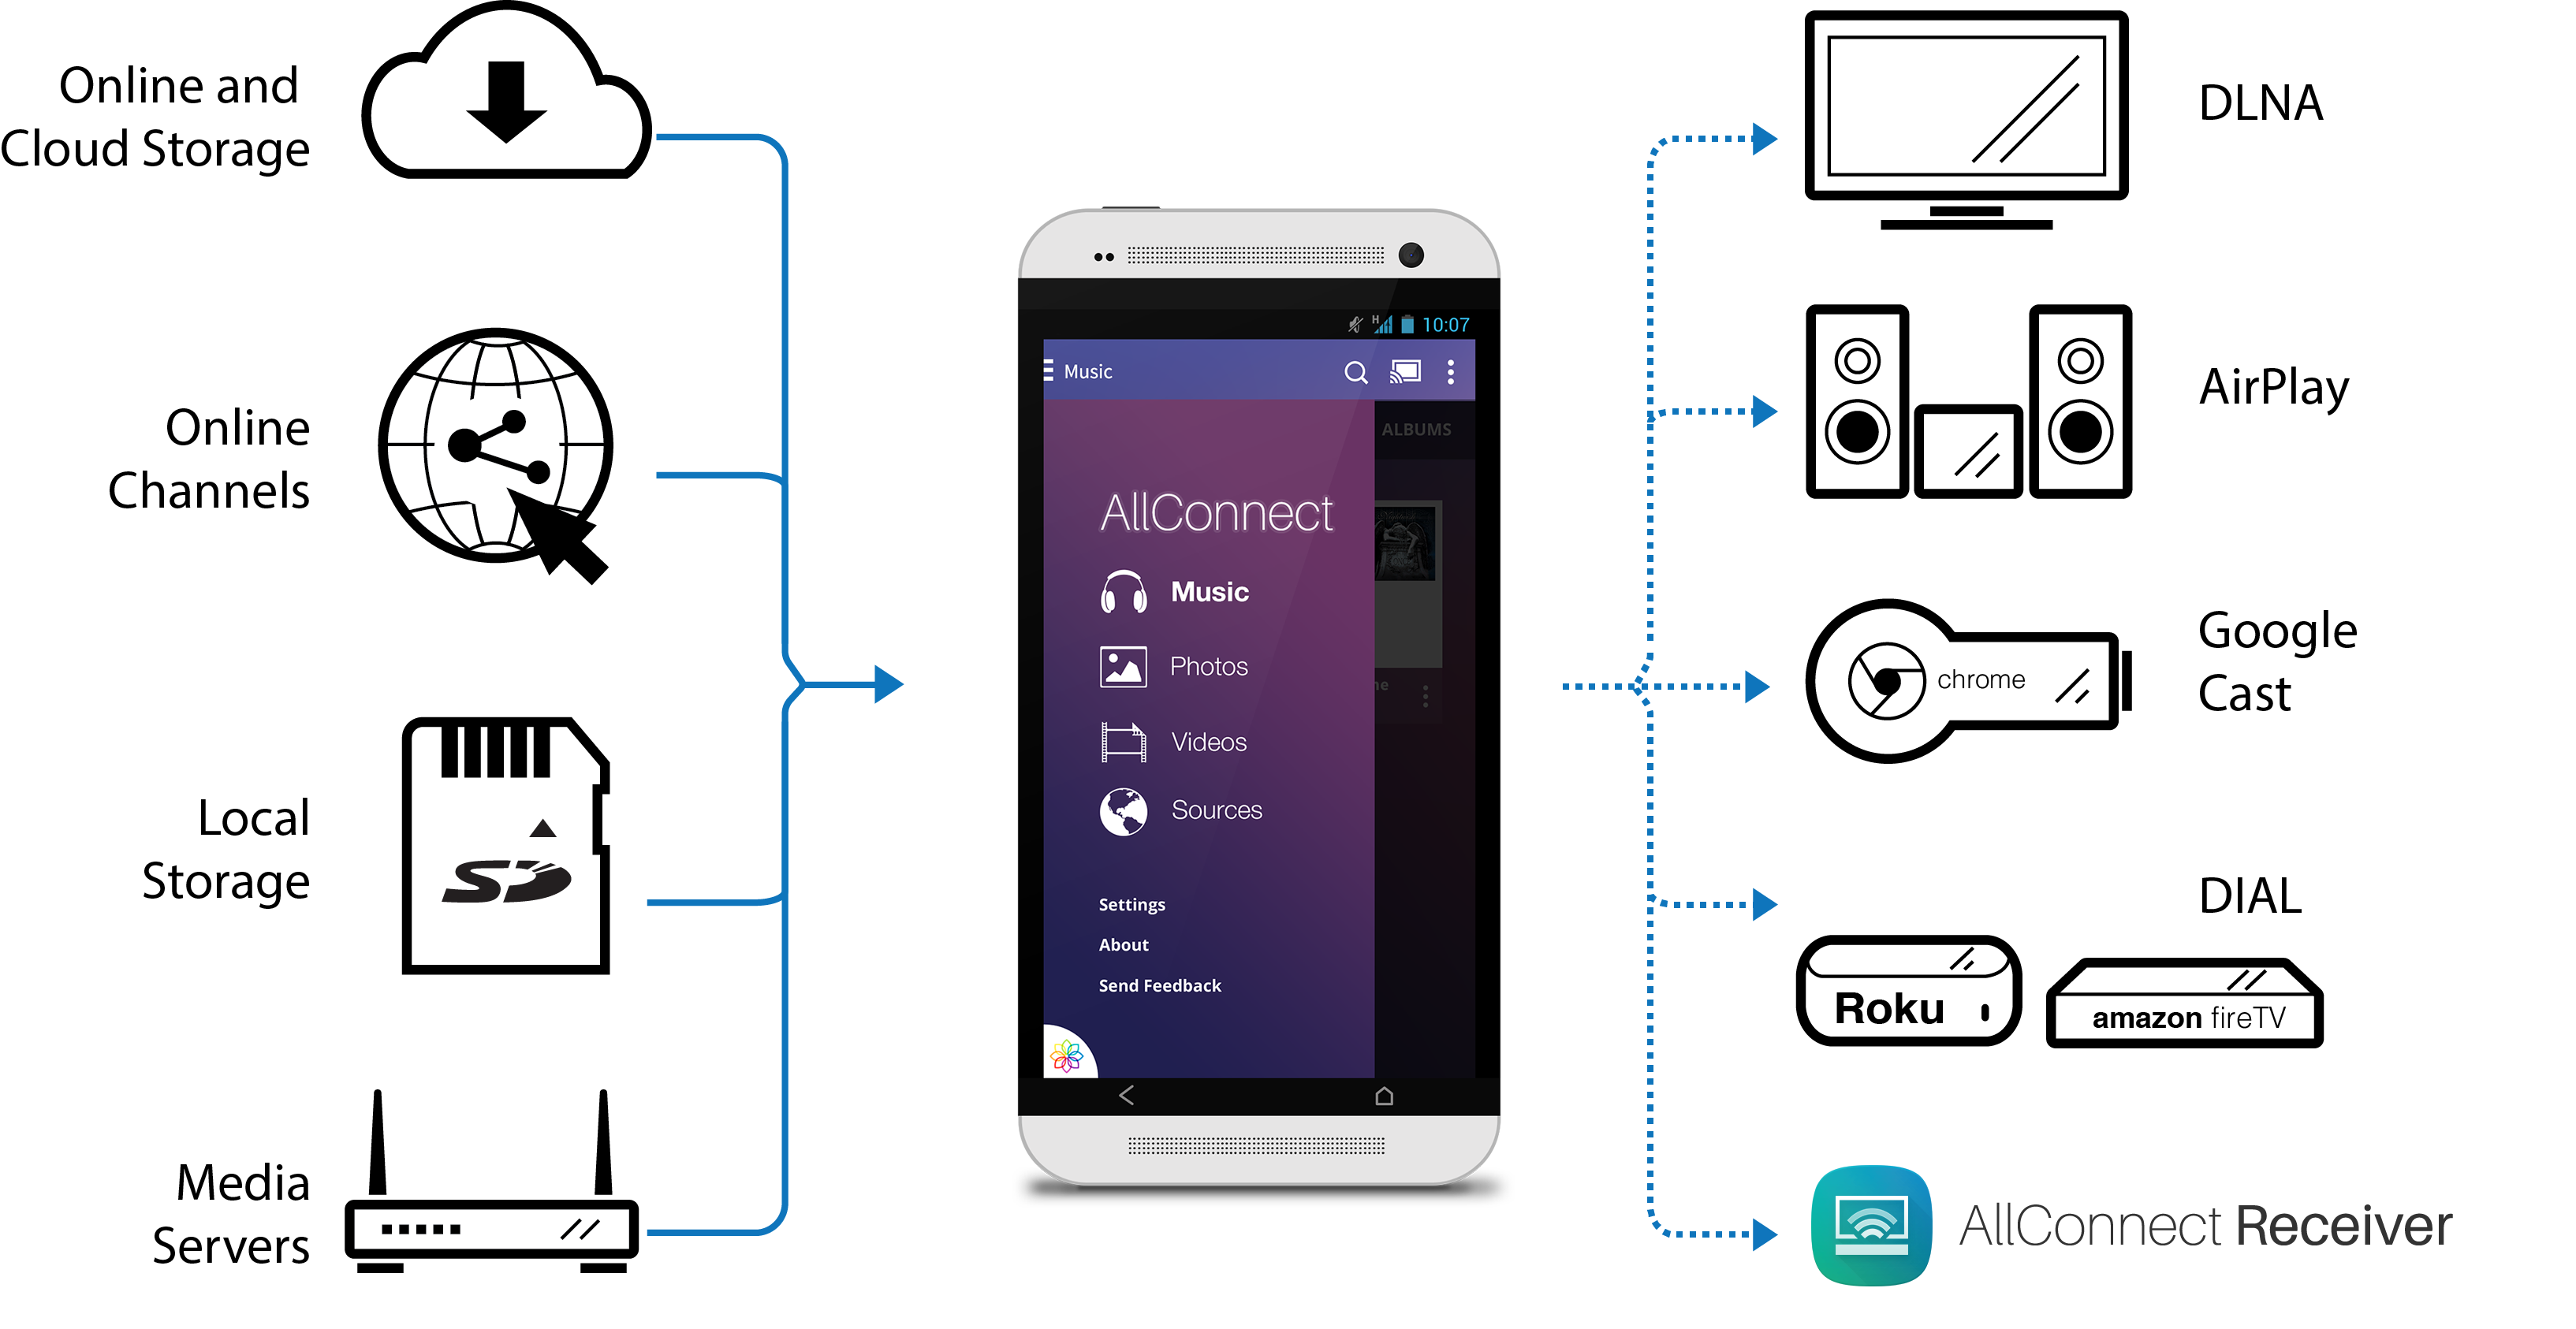
\includegraphics[height=8cm]{charts/allconnect-app}
\caption{Application UX design \label{chart5}}
\end{figure}

\subsection{Features}
The Android application we developed can handle most multimedia devices in a typical home networking. It has various features that make it a useful and universal solution for multimedia home networking.\\
\\
Firstly, the app itself is a multimedia player. All the media stored locally on the phone storage, all the media located in the DLNA media servers can be browsed and played on the phone.\\
\\
Secondly, the application is fully compatible with AirPlay, DLNA, Chromecast and FireTV receiver devices. All devices can be discovered as renderer devices.\\
\\ 
Thirdly and most importantly, the application make the DLNA media server works together with all kind of receivers regardless of protocol used. The app served as a bridge of different multimedia receivers and media sources.\\
\\
Last, YouTube and other on-line channels like Vimeo and Facebook are supported as media source. These content can be streamed regardless of protocol to all supported receivers that are connected to home network.

\subsection{Extensibility}
Streambels has embedded a media streaming server for local files and streaming proxy for bridging the gap between online resources and home networking. By using built-in proxy, Streambels is able to share on-line resources from Internet to devices in home networking environment. \\
\\
New service providers and content providers can integrate home networking support to their product easily by just sending formatted intent to our application following our guideline. The proxy will automatically bridge the gap between internet and home netowrk.\\
\\
The proxy system enables a huge extensibility possibility, which makes it possible to connect home networking to Internet or Cloud Services.\\
\\
In the future we could also develop a Software Development Kit (SDK) to make this technology even directly be used by other application builders.
\subsection{Test methodology}
Software testing is extremely important for a modern IT project. Buggy implementation may kill the product in the very beginning. Through testing we could assure the performance and stability of our product. Before the final releasing to App store, the application needs to be thoroughly tested.\\
\\
These tests include unit test, integration test and functional test.
Unit tests were written while coding, when each class was finished, unit tests would be written for each method. We also set up an continuous integration server so that each time we commit anything to the git repository, full set of unit tests will be executed. If there were any failure in the unit tests, developer will be immediately notified. Integration tests were done in a way that we ensure each function module should work together with other modules in the system. Last, we listed all the possible use cases in paper and prepared a huge media base which contains all kind of media files. With all these preparations ready, manual tests were conducted before the app is finally released in the market.

\subsection{Evaluation methodology}
Experimental setup(TBD)\\
\\
Since the product is targeted to Android market and is directly used by end users, user feedback is really important to us for improving the product continuously. Email is used for normal communication between user and our support. A submission window is built inside the application, so that users can easily send feedback to us directly by Email.\\
\\
There is no perfect program, crashes sometimes happen. Thanks to Google, all crash reports are collected and showed inside developer console. This makes it a lot easier to track and debug our application.\\
\\
Inside Streambels, we also integrated Google's Analytics API. The API provided great convenience for us to collect number of users and sessions every day. Other information such as version of operating system, application version, active users helped us to achieve better insights to our users and helped us to market our application to more
people in the world.\\
\\
It is also interesting to see what kind of technologies are most used in their daily life. With the analytics SDK, we could trigger events when user select their receivers. After months of statistics, we have figured out the most popular standards and most popular online channels that user uses.\\
\\
These valuable information will in turn help our decision making on how we should improve our application. Some of these result will be discussed in chapter 4.